%Første egentlige afsnit i rapporten er indledningen, som skal få læseren til at forstå produktet (i modsætning til forordet, der handler om rapporten). Produktets faglige baggrund og produktets problemstilling beskrives her. I dette afsnit indsættes den konkrete problemformulering som I har udarbejdet på baggrund af et evt. projektoplæg. For at oprette fokus på produktet beskrives det samlede system, der er tænkt realiseret i projektet. Anvend illustrationer for at uddybe systemets funktionalitet for læseren. Beskrivelsen bør ligeledes fortælle, om systemet er bygget som en prototype eller som et endeligt produkt. Indledningen kan også beskrive vigtige begreber, definitioner, anvendte forkortelser m.m. Dette afsnit skal også indeholde en oversigt over, hvilke projektdeltagere der har hvilke produktmæssige hovedansvarsområder. En sådan kan med fordel beskrives i en tabel.
\newpage
\chapter{Introduction}
In recent years, there has been an increased focus on autonomous vehicles, both by land, sea, and air. Self-driving cars, drones, and automatic survey vessels are examples of this, and the trend seems to continue as the technology matures and becomes accepted more broadly in society.

Autonomy ensures repeatability, reduces many categories of risk, and - by definition - eliminates the error-prone human element from the equation, often leading to much better results and favourable cost. 

This project focuses on developing a system that can survey an area of the sea from inputs in a UI autonomously, thus removing the need for route planning by surveyors, enabling them to focus on data analysis rather than data acquisition. 

An overview of the system is seen in figure \ref{table:rich_image}.

As such, the system requires a number of components. 

A UI which allows the user to set up parameters such as the width of the survey equipment, and specify an area on a map to cover in an intuitive way. The map will be updated continually if a network is available, otherwise an offline version of the most important quadrants is used.

A controller which takes care of navigation and autopiloting based on user commands, parameters, and GPS data. Relevant information such as position of the ship, planned route, and completed route are then shown in the UI.

A server which hosts the website and writes/reads data to/from the website and controller.

A prototype ship with a rudder and thruster and hull space for the controller unit, GPS receiver, battery, motor controller(s).

A command computer to communicate with the controller and view the UI.

\begin{figure}[H]
	\centering
	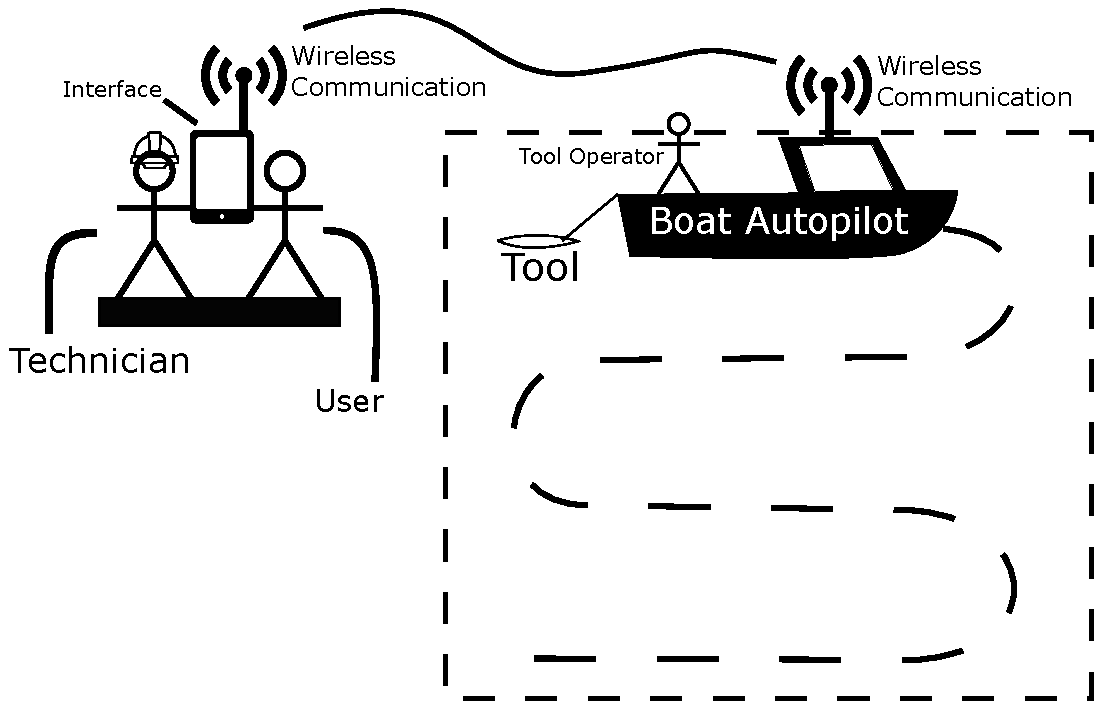
\includegraphics[width=1\linewidth]{rich_image}
	\caption{Rich image of system}
	\label{table:rich_image}
\end{figure}

\section{Areas of responsibility}
Table \ref{table:overview} shows the general outline of which group member had the responsibility for which area. As seen, each section was a shared effort, but generally not equally time-consuming for each developer.

Requirements specification, architecture, defining the acceptance test, and choosing system components was done as a collaborative effort, only when the project entered the design and implementation phase did tasks become individual. 

Tables \ref{table:website}, \ref{table:controller}, and \ref{table:hardware} shows a more detailed view of these responsibilities.

\begin{table}[H]
\centering
\begin{tabular}{|c|c|}
\hline 
\textbf{Overview} & \\ 
\hline 
\textbf{Area} & \textbf{Developer} \\ 
\hline 
Website & Troels and Nicolai \\ 
\hline 
Controller & Troels and Nicolai \\ 
\hline 
Hardware & Troels and Nicolai \\ 
\hline 
\end{tabular} 
\caption{Overview of areas of responsibility}
\label{table:overview}
\end{table}

\begin{table}[H]
\centering
\begin{tabular}{|c|c|}
\hline 
\textbf{Website} & \\ 
\hline 
\textbf{Task} & \textbf{Developer} \\ 
\hline 
Initial setup in bootstrap & Nicolai \\ 
\hline 
Edit parameters & Troels and Nicolai \\ 
\hline 
Coverage & Nicolai \\ 
\hline 
Point to point & Troels \\ 
\hline 
Status & Nicolai \\ 
\hline 
\end{tabular} 
\caption{Areas of responsibility for the website}
\label{table:website}
\end{table}

\begin{table}[H]
\centering
\begin{tabular}{|c|c|}
\hline 
\textbf{Controller} & \\ 
\hline 
\textbf{Class} & \textbf{Developer} \\ 
\hline 
JSONReceiver & Nicolai \\ 
\hline 
Navigation & Troels \\ 
\hline 
Autopilot & Nicolai \\ 
\hline 
DCMotor & Troels and Nicolai \\ 
\hline 
Servo & Troels and Nicolai \\ 
\hline 
JSONTransmitter & Troels \\ 
\hline 
GPS & Nicolai \\ 
\hline 
Unit tests & Troels and Nicolai \\ 
\hline 
Integration tests & Troels \\ 
\hline 
\end{tabular} 
\caption{Areas of responsibility for the controller}
\label{table:controller}
\end{table}

\begin{table}[H]
\centering
\begin{tabular}{|c|c|}
\hline 
\textbf{Hardware} & \\ 
\hline 
\textbf{Area} & \textbf{Developer} \\ 
\hline 
Component analysis and acquisition & Troels and Nicolai \\ 
\hline 
Design & Nicolai \\ 
\hline 
Implementation & Nicolai \\ 
\hline 
\end{tabular} 
\caption{Areas of responsibility for the hardware}
\label{table:hardware}
\end{table}